\section{Experiments and Results}
\label{sec:experiments}
% ====================================================================

We evaluate the DA2 pipeline through three experiments:
(1)~establishing upper-bound baselines with ground-truth sensing,
(2)~closing the gap between estimated and ground-truth depth by
varying model capacity and terrain texture, and
(3)~testing domain invariance under visual perturbations.
We report \emph{success rate} (fraction of episodes completing the
full course) and \emph{progress ratio} (mean fractional distance
along the course before termination), both averaged over 256
episodes.

% ====================================================================
\subsection{Baselines}
\label{sec:baselines}

We start by establishing upper bounds for the privileged teacher and the ground-truth depth sensing student (GT-depth).
The privileged teacher achieves near-perfect success across all gap difficulties, shown in Table~\ref{tab:baselines}.

\begin{table}[h]
  \centering
  \caption{Baseline success rates on gap terrain (\%).}
  \label{tab:baselines}
  \small
  \begin{tabular}{@{}lcccc@{}}
    \toprule
    & Row~0 & Row~1 & Row~2 & Row~3 \\
    \midrule
    Scandots teacher & 98.5 & 100.0 & 99.0 & 98.5 \\
    GT-depth student & 94.5 & 94.5 & 89.1 & 87.5 \\
    Zero-depth ablation & 8.0 & 2.0 & 0.0 & 0.0 \\
    \bottomrule
  \end{tabular}
\end{table}

The GT-depth student, receiving simulator depth images,
achieves $\geq$87\% success on all rows, confirming the CNN--GRU
architecture extracts sufficient geometry from a single depth viewpoint.
A zero-depth ablation (all depth pixels set to zero)
drops success to 8\%, verifying the policy relies on depth
rather than exploiting proprioceptive heuristics.

Figure~\ref{fig:teacher_training} shows training dynamics for both
baseline stages. Reward rises steeply as the policy masters flat terrain, then continues
climbing as the adaptive curriculum exposes progressively harder
obstacles. The GT-depth student's
distillation loss drops quickly but success climbs gradually, reflecting the difficulty of recovering the
teacher's behavior from a single depth viewpoint.


\begin{figure}[h]
  \centering
  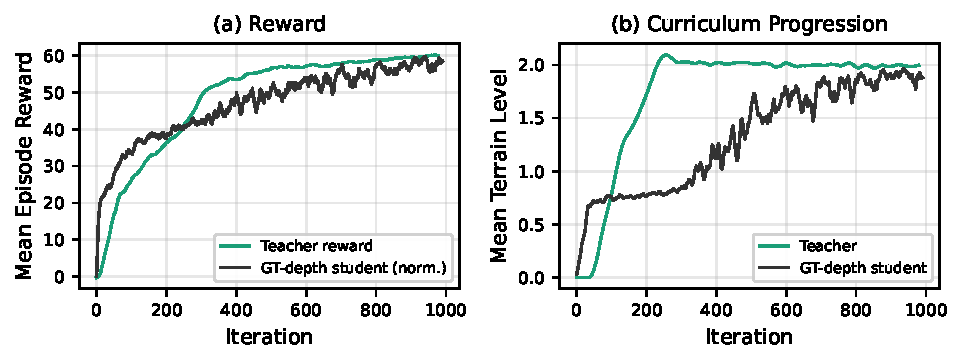
\includegraphics[width=\linewidth]{figures/teacher_training.pdf}
  \caption{Baseline training curves.}
  \label{fig:teacher_training}
\end{figure}


% ====================================================================
\subsection{Parkour from Estimated Depth}
\label{sec:da2_results}

We now determine whether parkour can be achieved from estimated
depth. Starting from the GT-depth setup, we first replace simulator
depth with DA2-small. 
As shown in Table~\ref{tab:da2_main}, 
DA2-small achieves success on Row~0 and 1, but fails completely on Rows~2 and 3.
Switching to DA2-base results in promotion to Row 3, but it still falls well short of
GT-depth on the hardest rows.

% TODO: visuals of row 1-4
% TODO: visuals of with and without texture including DA2s perception of obstacles
% TODO: depth quality metric?

The remaining limitation is the visual input. On untextured terrain,
the gap boundary provides weak monocular cues, so the depth estimate is
ambiguous. As shown in 
Table \ref{tab:da2_main},
adding checkerboard terrain texture makes the gap geometry
visible and closes most of the remaining gap to GT-depth.

Figure~\ref{fig:student_success} shows the same pattern during
training: the untextured models plateau early, while DA2-base +
texture continues improving and approaches the GT-depth student.
Breaking success down by obstacle type shows most of the gain comes from gap traversal; stairs and hurdles are much
less sensitive to texture because their geometry remains visible
without ground texture.


\begin{table}[h]
  \centering
  \caption{Policy success (\%) as model scale and terrain texture are added
  to the estimated-depth pipeline }
  \label{tab:da2_main}
  \small
  \begin{tabular}{@{}lcccc@{}}
    \toprule
    Configuration & Row~0 & Row~1 & Row~2 & Row~3 \\
    \midrule
    GT-depth baseline & 94.5 & 94.5 & 89.1 & 87.5 \\
    DA2-small & 56.3 & 33.6 & --- & --- \\
    DA2-base & 68.4 & 83.2 & 26.6 & 0.8 \\
    DA2-base + texture & 87.5 & 93.0 & 87.1 & 80.5 \\
    \bottomrule
  \end{tabular}
\end{table}

\begin{figure}[h]
  \centering
  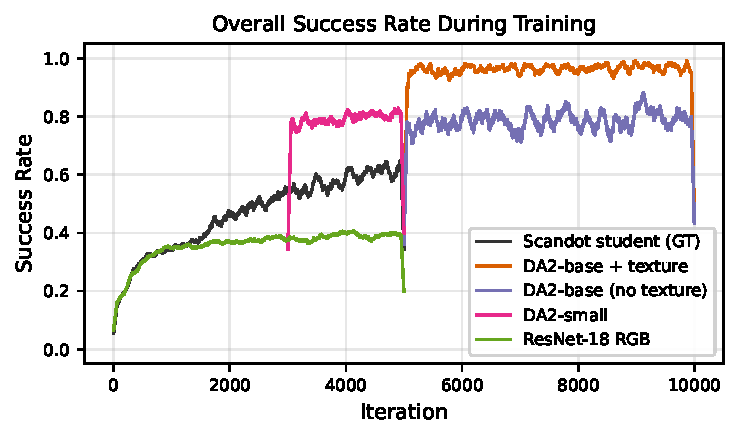
\includegraphics[width=\linewidth]{figures/student_success_comparison.pdf}
  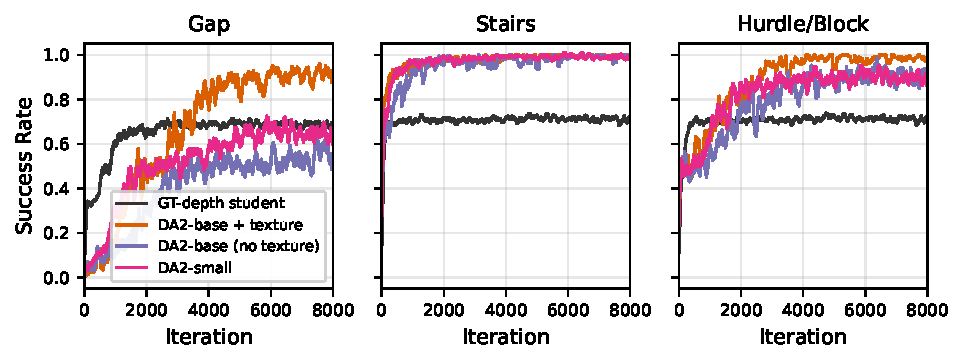
\includegraphics[width=\linewidth]{figures/per_obstacle_success.pdf}
  \caption{Overall and per-obstacle success rate during student training.}
  \label{fig:student_success}
\end{figure}

% ====================================================================
\subsection{Domain Invariance}
\label{sec:domain}

Having established strong parkour performance from estimated depth,
we now test whether DA2 provides invariance to the visual domain
shifts encountered in sim-to-real transfer. We apply perturbations
at test time only to the trained student,
covering two categories of shift: replacing the training
checkerboard with alternative surfaces, and applying brightness or per-channel color
jitter to the rendered RGB before DA2 inference.

\begin{table}[h]
  \centering
  \caption{Test-time success under visual perturbations.}
  \label{tab:domain_inv}
  \small
  \begin{tabular}{@{}p{3.6cm}rrr@{}}
    \toprule
    Perturbation & Succ. & Prog. & $\Delta$ \\
    \midrule
    Baseline (checkerboard) & 96.9\% & .948 & --- \\
    \midrule
    \multicolumn{4}{@{}l}{\textit{Texture replacement (structured)}} \\
    \quad Bricks & 89.8\% & .908 & $-$7.1 \\
    \quad Noise & 78.1\% & .843 & $-$18.8 \\
    \midrule
    \multicolumn{4}{@{}l}{\textit{Texture removal (featureless)}} \\
    \quad No texture & 18.0\% & .437 & $-$78.9 \\
    \quad Solid red & 23.4\% & .471 & $-$73.5 \\
    \quad Solid blue & 14.8\% & .417 & $-$82.1 \\
    \quad Flat grey & 18.0\% & .456 & $-$78.9 \\
    \midrule
    \multicolumn{4}{@{}l}{\textit{Color / brightness jitter}} \\
    \quad Brightness $\pm$30\% & 95.3\% & .937 & $-$1.6 \\
    \quad Brightness $\pm$60\% & 94.5\% & .935 & $-$2.4 \\
    \quad Color $\pm$15\% & 91.4\% & .914 & $-$5.5 \\
    \quad Color $\pm$30\% & 76.6\% & .816 & $-$20.3 \\
    \midrule
    \multicolumn{4}{@{}l}{\textit{Combined}} \\
    \quad Mild (bricks+b30+c15) & 82.0\% & .862 & $-$14.9 \\
    \quad Extreme (noise+b60+c30) & 63.3\% & .747 & $-$33.6 \\
    \bottomrule
  \end{tabular}
\end{table}

Table~\ref{tab:domain_inv} shows a clean separation between the two
shift types. The student is robust to the perturbations most
relevant to deployment: brightness jitter costs at most 2.4~pp,
moderate color jitter 5.5~pp, and switching to a brick texture only
7.1~pp. Performance degrades gracefully under structured noise and
combined mild perturbations, retaining 78--82\% success.

Featureless surfaces, by contrast, cause catastrophic failure
($-73$ to $-82$~pp). This is not a domain-invariance failure but a
fundamental input requirement: monocular depth estimation needs
visual features to infer geometry. Real-world surfaces (concrete,
wood, soil) all carry natural texture, so this regime is an
artifact of simulation rather than a deployment concern.
